%======================================================
% This file is part of
%  AMCOS_booklet 
% Version 1.1 (04/07/2019)
% A LaTeX template for conference books of abstracts
%
% This template is available at:
% https://github.com/maximelucas/AMCOS_booklet
%
% License: GNU General Public License v3.0
%
% Authors:
% Maxime Lucas (ml.maximelucas@gmail.com)
% Pau Clusella
%=======================================================

\documentclass[openany, twoside, parskip=half, 12pt, a4, BCOR=2cm, open=any]{scrbook}

\input{preamble}
\input{preamble_booklet}
	
\begin{document}

% COVER PAGE
%--------------------------------------------------------------------
\includepdf{PESGRE_Cover.pdf}	% our cover was produced with canva.com
	
	
% BLANK PAGE
%---------------------------------------------------------------------
\mbox{}
\thispagestyle{empty}
\vfill
\begin{center}
	\ifOnline
	The electronic version of this booklet can be found at: \\
	https://pesgre2025.org/
	\else
	This is the short version of the booklet for print use. Full abstracts with all authors, references, and figures can be found in the electronic version at \url{http://ieee-pesgre.org/}
	\fi % end if
	\\[20pt] % Please cite us by keeping the following line.
	The open-source \LaTeX{} template, AMCOS\_booklet, used to generate this booklet is available at \url{https://github.com/maximelucas/AMCOS\_booklet}
\end{center}

\newpage

% TABLE OF CONTENTS 
%---------------------------------------------------------------------
\tableofcontents

% ABOUT
%---------------------------------------------------------------------
\chapter{About PESGRE 2025}

%{\small \textcolor{myblue}{This is a generic version of the real AMCOS conference booklet for which this \LaTeX{} template was generated. All information about the use and distribution of this template, and all related codes, can be found at \url{https://github.com/maximelucas/AMCOS\_booklet}.}}

%\section{AMCOS}
IEEE PESGRE 2025 is the 4th IEEE International Conference on Power Electronics, Smart Grid and Renewable Energy, bringing together researchers, industry professionals and educators to discuss advances in power conversion, electric transportation and sustainable energy systems. The theme of this edition of conference is “Power Electronics and Renewable Energy for Sustainable Development”, being held during 18th - 21st December 2025 at Indian Institute of Technology Dharwad, Dharwad, Karnataka, India.

The conference covers core areas in power electronics, smart grids, renewable energy, electric vehicles, energy storage, and modern power systems, including policy and standards. It also includes special sessions on emerging topics and dedicated Students and Young Professionals (SYP) activities to promote early-career research and networking in the global power and energy community.

IEEE PESGRE is the biennial flagship Conference of IEEE Kerala Section, IEEE IA/IE/PELS Joint Chapter Kerala and IEEE Industry Applications Society. The technical co-sponsors of the conference include IEEE Power Electronics Society, IEEE Industrial Electronics Society, and IEEE Power \& Energy Society.



\hrule \n
\section{Organizing committee}
\begin{center}
\begin{tabular}{ll}

\multicolumn{2}{c}{\textbf{Co-General Chairs}}\\
\multicolumn{2}{l}{\textbf{Satish Naik Banavath}, Indian Institute of Technology Dharwad, Karnataka, India}\\
\multicolumn{2}{l}{\textbf{Dmitri Vinnikov}, Tallinn University of Technology, Estonia}\\
\multicolumn{2}{l}{\textbf{Sheldon Williamson}, Ontario Tech University, Canada}\\
& \\
& \\
\textbf{Patron} & \textbf{Venkappayya R Desai}, Director, IIT DHARWAD \\
& \\
\multirow{6}{*}{\textbf{Honorary Chairs}}
& \textbf{Andy Knight}, President, IEEE IAS \\
&\textbf{ Brad Lehman}, President, IEEE PELS \\
& \textbf{Milos Manic}, President, IEEE IES \\
&\textbf{ Shay Bahramirad}, President, IEEE PES \\
&\textbf{ Muhammed Kasim S}, Chair, IEEE Kerala Section \\
&\textbf{ Vasanthi V}, Chair IA/IE/PELS Jt. Chapter Kerala Section \\
& \\
\multirow{4}{*}{\textbf{Technical Program Chairs}} & \textbf{Abhijit Kshirsagar}, IIT Dharwad, India \\
&\textbf{ Andrii Chub}, Tallinn University of Technology, Estonia \\
&\textbf{ Rajendra Singh}, Clemson University, Clemson USA \\
&\textbf{ Bijuna Kunju K}, TKMCE, Kollam, India \\
& \\

\multirow{3}{*}{\textbf{Special Session Chairs}} & \textbf{Deepak Ronanki}, IIT Madras, India \\
& \textbf{Sertac Bayhan}, Hamad Bin Khalifa University, Qatar \\
& \textbf{Sairaj Dhople}, University of Minnesota, USA\\

& \\

\multirow{3}{*}{\textbf{Publication Chairs}} &  \textbf{Srinivas Bhaskar Karanki}, IIT Bhubaneswar, India \\
& \textbf{Amarkumar Ayodhyasingh Kushwaha}, IIT Dharwad, India \\
& \textbf{Jaison Mathew}, Government Engineering College\\
& Thrissur, Kerala, India \\
& \\
\multirow{4}{*}{\textbf{Publicity Chairs}} & \textbf{Animesh Kumar Sahoo}, IIT Dharwad, India \\
& \textbf{Naga Brahmendra}, IIT Palakad, India \\
& \textbf{Biju K}, APJ Abdul Kalam Technological University, Kerala, India \\
& \textbf{Kalpana R}, NIT Karnataka, India \\
& \\
\multirow{3}{*}{\textbf{Finance Chairs}} & \textbf{Satish Naik Banavath}, IIT Dharwad, India \\
&\textbf{ Prathyasa Bhui}, IIT Dharwad, India \\
& \textbf{Sabiq P V}, Treasurer, IEEE Kerala Section, India \\
\end{tabular}
\end{center}

\begin{center}
\begin{tabular}{l}
\multicolumn{1}{c}{\textbf{International Advisory Board}}\\
 \\
S C Srivasthava, IIT Kanpur, India\\ 
Amit Kumar Gupta, Rolls Royce, Singapore\\ 
Bhim Singh, IIT Delhi, India\\ 
C. Chakraborty, Indian Inst. of Technology Kharagpur, India\\ 
Chun Che Fung, Director, IEEE R10\\ 
Drazen Dujic, EPFL, Switzerland\\ 
Enrique Romero Cadaval, University of Extremadura, Spain\\ 
Frede Blaabjerg, Aalborg University\\ 
G. Bhuvaneswari, Mahindra University, India\\ 
Giovanni De Carne, KIT, Germany\\ 
Gopakumar K, IISc Bangalore, India\\ 
Holtz, University of Wuppertal, Germany\\ 
J. Rabkowski, Warsaw University of Technology, Poland\\ 
Johann W. Kolar, ETH Zurich, Zurich, Switzerland\\ 
Kaushik Rajashekara, University of Houston, Texas, USA\\ 
L Umanand, IISc Bangalore, India\\ 
Mariusz Malinowski, Warsaw University of Technology, Poland\\ 
Pragasen Pillai, Concordia University, Canada\\ 
Prasad Enjeti, Texas A\&M University, USA\\ 
S S Murthy, BoG Member, IIT Dharwad\\ 
Subba Reddy B, IISc Bangalore\\ 
S. Norrga, KTH Royal Institute of Technology, Sweden\\ 
Sameer S M, Secretary, IEEE R10\\ 
Samir Kouro, Universidad Tecnica Federico Santa Maria Valparaiso, Chile\\ 
Sanjib Panda, NUS Singapore\\ 
Suresh Nair, Immediate Past Chair, IEEE India Council\\ 
Vivek Agarwal, IIT Bombay, India\\ 
V. Fernão Pires, Polytechnic Institute of Setubal, Portugal\\ 
 \\
\multicolumn{1}{c}{\textbf{Student and Young Professionals Chairs}}\\
Chathurika S. Wickramasinghe, USA \\
Jo\~ao Carvalho Neto, Brazil\\
Edivan Laercio Carvalho da Silva, Tallinn University of Technology, Estonia \\
Filipe Pinarello Scalcon, University of Calgary, Canada \\
Sai Ram Boggavarapu, IIT Dharwad, India \\
\end{tabular}
\end{center}


\chapter{Welcome Message}

On behalf of the Organizing Committee and the Technical Program Committee,
we are delighted to welcome you to the \textbf{4th IEEE International Conference on Power Electronics, Smart Grid, and Renewable Energy (IEEE PESGRE 2025)}, hosted at the vibrant campus of Indian Institute of Technology Dharwad, Karnataka, India, from December 18 - 21, 2025.

IEEE PESGRE is the biennial flagship conference of \textbf{IEEE Kerala Section, IEEE IA/IE/PELS Joint Chapter Kerala}, and the \textbf{IEEE Industry Applications Society}, with financial co-sponsorship from these bodies. Technical co-sponsors include the \textbf{IEEE Power Electronics Society}, \textbf{IEEE Industrial Electronics Society}, and \textbf{IEEE Power \& Energy Society}.

The theme for this edition is \textbf{``Power Electronics and Renewable Energy for Sustainable Development }. The conference will spotlight cutting-edge technologies, strategies, and challenges in power electronics, renewable energy, electric vehicles, grid integration, and smart grid solutions. IEEE PESGRE 2025 serves as a global platform for exchanging ideas, presenting technical innovations, and discussing current trends and future perspectives in areas such as power converter topology, control techniques, grid integration, etc.

This edition conference reflects a truly international scope, with participants and presentations from \textbf{15 countries}, which includes, Canada, China, Estonia, Germany, India, Israel, Italy, Norway, the Netherlands, New Zealand, Poland, UAE, USA, etc. This shows the increasing popularity of the conference by underscoring the global commitment to advancing energy systems.

Out of \textbf{400 submissions, 210 papers} were accepted after a rigorous review process with three reviewers per paper involving \textbf{20 track chairs} and \textbf{350 expert reviewers} from different countries.  Finally, a total of \textbf{179 camera-ready papers} will be presented across 30 technical oral sessions.
%
The program features:
%
%\parbox{\linewidth}{
\begin{itemize}
\setlength{\itemsep}{0pt}        % Space between items
\setlength{\parskip}{0pt}        % Space between paragraphs within an item
\setlength{\parsep}{0pt}         % Additional paragraph separation
\item 4 Keynote Addresses
\item 1 IES SYPA Keynote
\item 4 Tutorials
\item Two Women in Engineering (WiE) Sessions
\item PELS Young Professional Mentorship Program
\item Panel Discussion
\item Five Industry Sessions
\item Three oral presentation sessions covering 180 papers and 
\item Cultural events 
\end{itemize}
%}

We are proud to note the strong industry presence at PESGRE 2025, highlighting the growing real-world relevance of power electronic technologies and the importance of academia-industry collaboration. Together, we are shaping the future of sustainable energy systems. This belief is strengthened by our sponsors who are from different industrial sectors, related to manufacturers of power supplies and testing equipment, defence systems, renewable energy, battery technology, simulation tools, etc. 
Our sincere appreciation goes to the sponsors for their invaluable support:
\begin{itemize}
\setlength{\itemsep}{0pt}        % Space between items
\setlength{\parskip}{0pt}        % Space between paragraphs within an item
\setlength{\parsep}{0pt}         % Additional paragraph separation
	\item \textbf{Title Sponsor}: JSCGI Private Limited
	\item \textbf{Platinum Sponsors}: Pragna Microdesigns and Defence Research and Development Organisation (DRDO)
	\item \textbf{Gold Sponsors}: Convergent Technologies + Tektronix
	\item \textbf{Silver Sponsors}: Karnataka Renewable Energy Development Limited (KREDL), OPAL-RT Technologies, and AARJAY International
	\item \textbf{Bronze Sponsors}: Charge House, HIOKI, Typhoon HIL, MathWorks, CDAC, and COMSOL
	\item \textbf{Other Sponsors}: Amara Raja Group, IFB, Reliamotive Labs, FLUKE, and Keysight
\end{itemize}



We extend our heartfelt gratitude to the Technical Program Committee chairs, track chairs, and reviewers for ensuring the high technical quality of this event, and to the authors, whose innovative contributions form the core of this conference.
Finally, as we gather to share knowledge and explore innovations, let us remember our common mission: building resilient, efficient, and sustainable energy systems. Power electronic technologies are at the heart of this transformation, and your participation is vital in shaping the future.
We encourage you to take full advantage of networking opportunities—during technical sessions, coffee breaks, and social events. 
We look forward to having you all here and have an inspiring, productive, and memorable week in Dharwad.

\vspace{-2mm}
\begin{center}
	\begin{tabular}{ccccc}
		\centering
		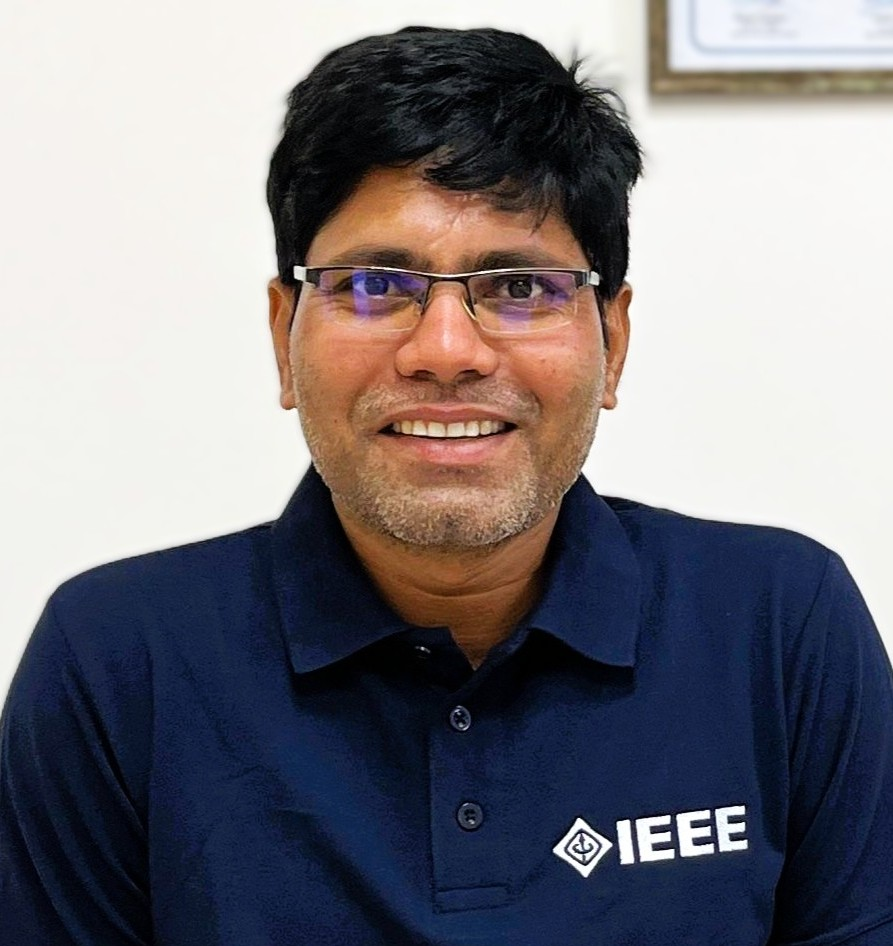
\includegraphics[width=35mm]{images/gc_satish.jpg} & \hspace{10mm}
		& 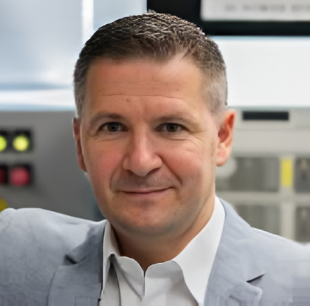
\includegraphics[width=35mm]{images/gc_dimitri.png} & \hspace{5mm}
		&  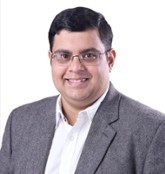
\includegraphics[width=35mm]{images/gc_sheldon.jpeg}\\
		Dr. Satish Naik & \hspace{10mm}
		& Dr. Dmitri Vinnikov & \hspace{10mm}
		&  Dr. Sheldon Williamson\\
		& & & & \\
		\multicolumn{5}{c}{Co-General Chairs, IEEE PESGRE 2025}
	\end{tabular}
\end{center}



% TIMETABLE 
%---------------------------------------------------------------------
\chapter{Schedule}
%Please check website for updated schedule: \url{https://pesgre2025.org/}
%
\begin{center}
\includegraphics[width=0.83\linewidth]{Schedule.pdf}	
\end{center}

%CT: Contributed Talk, IS: Invited Speaker, KL: Keynote Lecture, IT: Invited Talk.
%\input{timetable.tex}

% TALKS 
%---------------------------------------------------------------------
\chapter{Keynote Talks}
%\begin{abstract}{Title}{%
%		Speaker}{%
%		University}{%
%		\KLtag}
%Bio
%\end{abstract}

\begin{abstract}{Keynote 1: Interlinking hybrid distribution transformer for hybrid power grids}{%
		Prof. Mariusz Malinowski}{%
		Professor at the Institute of Control and Industrial Electronics, WUT, Poland.
	}{%
		\KLtag}
	\textbf{About the Speaker}:
	Professor Mariusz Malinowski received his Ph.D. and D.Sc. degrees in electrical engineering from the Warsaw University of Technology (WUT), Poland. He has authored over 200 technical papers and seven books. His research focuses on the control and modulation of grid-side converters, multilevel converters, smart grids, and renewable energy systems. He has received numerous awards, including the IEEE IES David Irwin Early Career Award, IEEE IES Bimal Bose Energy Systems Award, and the Polish Prime Minister Award. He is a Fellow of IEEE and a member of the Polish Academy of Sciences.
	
\end{abstract}

\begin{abstract}{Keynote 2: Brushless Field-excitation Systems for Motors in Electric Vehicles}{%
		Prof. Baylon G. Fernandes}{%
		Professor at the Department of Electrical Engineering, IIT Bombay, India.}{%
		\KLtag}
	\textbf{About the Speaker}:
	Professor Baylon G. Fernandes received the B.Tech. degree from the National Institute of Technology Karnataka, Surathkal, India, in 1984, the M.Tech. degree from the Indian Institute of Technology Kharagpur, India, in 1989, and the Ph.D. degree from the Indian Institute of Technology Bombay (IIT Bombay), India, in 1993, all in electrical engineering. Since 1998, he has been with the Department of Electrical Engineering, IIT Bombay, where he is currently a Professor. From 2015 to 2020, he served as the Chairman of the Department. He is a Principal Investigator of the National Centre for Photovoltaic Research and Education and the National Centre of Excellence in Technology for Internal Security at IIT Bombay. His research interests include power electronic converters, motors for electric vehicles, and power electronic interfaces for non-conventional energy sources. Prof. Fernandes is a Senior Member of IEEE and serves as an Associate Editor for IEEE Transactions on Power Electronics.
\end{abstract}

\begin{abstract}{Keynote 3: Transformative Role of Power Electronics in Accelerating Economic Growth of Bharat}{%
		Prof. Rajendra Singh}{%
		Houser Banks Distinguished Professor at Clemson University, USA
	}{%
		\KLtag}
	\textbf{About the Speaker}:
	Professor Rajendra Singh is the Houser Banks Distinguished Professor in the Holcombe Department of Electrical and Computer Engineering and Automotive Engineering at Clemson University (CU). Inspired by Thomas Edison's vision of solar energy, he pursued his Ph.D. dissertation on Silicon Solar Cells during the 1973 energy crisis. Over the past 50 years, he has significantly contributed to the growth of the photovoltaic and semiconductor industries. With expertise in operations, project leadership, R\&D, product commercialization, and startups, Dr. Singh is dedicated to mitigating climate challenges through sustainable green electric power. He has authored or co-authored over 500 publications and edited more than fifteen conference proceedings. He has delivered over 60 keynote addresses and invited talks at national and international conferences. Dr. Singh is the founding technical chair of the IEEE DC Microgrid Conference and currently serves as Chair of the IEEE Power and Energy Society Committee on End-to-End DC Power. He holds six patents, with technologies from his lab licensed for commercialization. Recognized with numerous national and international awards, he was named one of the ten Global Champions of Photovoltaics by Photovoltaics World in 2010. In 2014, he was honored by US President Barack Obama as a White House 'Champion of Change for Solar Deployment.' In 2019, he received the Hind Rattan (Jewel of India) Award. Dr. Singh is a Fellow of IEEE, SPIE, ASM, and AAAS.
\end{abstract}

\begin{abstract}{Keynote 4: Solid State transformer: A Promising Technology Needing Many Breakthroughs}{%
		Prof. Drazen Dujic}{%
		Associate Professor and Head of the Power Electronics Laboratory at EPFL, Switzerland.
	}{%
		\KLtag}
	\textbf{About the Speaker}:
	Drazen Dujic received the Dipl. Ing. and MSc degrees from the University of Novi Sad, Serbia, and the PhD degree from Liverpool John Moores University, UK. He has worked as a Research Assistant at the University of Novi Sad, a Research Associate at Liverpool John Moores University, and in various roles at ABB Switzerland Ltd. Since 2014, he has been with EPFL. His research focuses on high-power electronic systems and high-performance drives. He has received multiple awards, including the Istvan Nagy Award (2024), the EPE Outstanding Service Award (2018), and the Isao Takahashi Power Electronics Award (2014). He is an IEEE Fellow.
\end{abstract}



\begin{abstract}{Keynote 5: Magnetic energy harvesting from overhead power lines}{%
		Alon Kuperman}{%
		Ben-Gurion University of the Negev, Israel}{%
		\KLtag}
	\textbf{About the Speaker}: Alon Kuperman (Senior Member, IEEE) is a Full Professor with the School of Electrical and Computer Engineering, Ben-Gurion University of the Negev, Beer-Sheva, Israel and the Director of Applied Energy Laboratory. He holds multiple international patents and owns an independent consultancy services company. He is also a co-founder of two start-up companies focusing on wireless power transfer. His research interests include all aspects of energy conversion and applied control.
\end{abstract}




\chapter{Tutorial Sessions}

\begin{abstract}{Tutorial – 1: From Prototype to Product Readiness: IndustrialDesign Considerations for Dual Active BridgeConverters}{%
		Dr. Shan, Dr. Aravind, Dr. Gourahari}{%
		Schneider Electric, Bangalore
	}{%
		\Tutorialtag}
	\textbf{Abstract}:
	The Dual Active Bridge (DAB) converter is a promising DC-DC converter topology for medium-high power applications, offering bidirectional power transfer, galvanic isolation, and high efficiency. While academic research emphasizes on novel modulation strategies, robust control methods, and efficiency improvement; the transition from a prototype to an industrial product requires a broader and more holistic perspective.
	
	In addition to core power electronics, this tutorial presents the design of a Three-Phase Dual Active Bridge (3ϕ-DAB) converter for industrial applications, emphasizing the broader requirements that define product readiness. Critical aspects such as thermal management, mechanical robustness, and electromagnetic compliance (EMC/EMI) significantly influence industrial viability. Equally important are Design for Manufacturing (DFM), Design for Assembly (DFA), and Design for Reliability (DFR), which ensure scalability, cost-effectiveness, and consistency in mass production. Reliability practices, including DMA, DFMEA, further strengthen product robustness and long-term performance. With rising labour costs, industries are increasingly dependent on robotic and automated assembly lines. Therefore, converter design must also be automation-friendly, supporting repeatable and reliable processes such as automated soldering, reflow compatibility. Considering all these factors, the converter design must ultimately adhere to competitive market requirements by achieving high efficiency while minimizing cost, weight, and volume.
	This tutorial intends to give a brief insight to all the above said factors taking the Three Phase DAB as an example.
\end{abstract}

\begin{abstract}{Tutorial 2: Wireless Charging of Electric Vehicles: Design and Implementation}{%
		Dr. Francesca, Dr. Calina}{%
		Assistant Professor, Eindhoven University of Technology (TU/e), The Netherlands}{%
		\Tutorialtag}
	\textbf{Abstract}:
	Let’s assume that you want to design and implement a wireless charging system based on initial specifications and requirements. Where do we start the process? How do we choose the coil topology, compensation network, and power conversion stages? How do you model tolerances and evaluate/predict performance ? 
	At the end of this tutorial lecture, the student will be able to:
	Define boundary conditions and make design choices for the subcomponents of the wireless charger.
	Optimize the system's parameters.
	Evaluate the design considering manufacturing tolerances and other non-idealities. 
	
	Delivery methods:
	Lecture with slides
	Guided design task
\end{abstract}

%Tutorial – 3: 
\begin{abstract}{Tutorial 3: Reliability and circularity in the future highly efficient and high-power density DC power electronic converters}{%
		Dr. Riccardo\textsuperscript{1}, Dr. Mattia\textsuperscript{1}, Dr. Husev\textsuperscript{2}}{%
		University of Bologna, Italy\textsuperscript{1}, Gdansk University of Technology, Poland\textsuperscript{2}}{%
		\Tutorialtag}
	\textbf{Abstract}:
	As the global energy landscape evolves toward decarbonization, electrification, and digitalization, the demand for highly efficient and compact DC power electronic converters continues to surge. These converters are pivotal in enabling next-generation applications across renewable energy systems, electric mobility, data centers, and aerospace technologies. However, achieving high power density and efficiency often brings challenges related to thermal management, component stress, and long-term system reliability.
	
	This keynote will explore the interplay between reliability and circularity in the design and operation of future power converters. It will examine recent advances in wide-bandgap semiconductors, intelligent control strategies, and modular topologies that address efficiency and density goals while also focusing on design for longevity, ease of maintenance, reuse, and lifecycle carbon footprint.
	
	Bridging academic insights with industrial relevance, the keynote will outline strategies for embedding circular economy principles into the converter lifecycle—spanning design, usage, and lifecycle assessment. Attendees will gain a forward-looking perspective on how engineering innovation and sustainable design practices can together pave the way for resilient, resource-efficient power electronics in a rapidly transforming energy ecosystem.
\end{abstract}


\begin{abstract}{Tutorial 4: SiC MOSFETs Based Power Electronics: Challengesand Opportunities}{%
		Prof. Sandeep Anand\textsubscript{1}, Dr. Abhinav\textsubscript{2}}{%
	IIT Bombay\textsubscript{1} and IIT Bhubaneswar\textsubscript{2}, India
}{%
		\Tutorialtag}
	\textbf{Abstract}:
	The transition from conventional silicon IGBTs to silicon carbide (SiC) MOSFETs
	is redefining modern power electronics by enabling faster switching and higher switching
	frequency operation. This tutorial will explore the fundamental need for higher switching
	frequencies to achieve reduced passive component size while considering overall system
	efficiency. We will delve into the I-V characteristics of SiC MOSFETs, their switching
	behaviour, and the impact of parasitic capacitances on switching losses. A detailed comparison
	between SiC MOSFETs and Si-IGBTs will highlight the clear performance advantages of
	wide-bandgap semiconductors, while also addressing critical design challenges.
	Attendees will gain insights into circuit-level issues such as dv/dt-induced false turn-on,
	EMI/EMC concerns, gate driver complexities, and the need for fast-acting short-circuit
	protection. We will also discuss key reliability concerns, including gate oxide and body diode
	degradation mechanisms. The tutorial will also include the medium-voltage applications of the
	SiC MOSFETs, where these challenges become even more pronounced. The session will
	conclude with a brief presentation of our recent research findings, offering practical
	perspectives and design recommendations. This tutorial aims to equip engineers and
	researchers with a clear understanding of both the opportunities and obstacles in harnessing the
	full potential of SiC MOSFETs in next-generation power electronic systems.
\end{abstract}


\chapter{List of Abstracts}

\begin{center}
	\Large NOTE: The latest schedule of Oral Presentations is available on the website at \url{http://pesgre2025.org}
\end{center}

%\section{Tuesday 20th}

% Definitions of custom environment used here can be found in preamble_booklet.tex file

% The following input commands automatically select the right version 
% (print or online) version of the abstract's .tex
% \type is defined in preamble_booklet.tex and equals:
% 'o' (online) or 'p' (print)


%\input{abstracts/tex/tp_tremblay}
%\input{abstracts/tex/t\type_fournier}
%\input{abstracts/tex/t\type_sato}
%\input{abstracts/tex/t\type_smith}
%\input{abstracts/tex/t\type_rodriguez}
%\input{abstracts/tex/t\type_jansen}
\section{Oral Session OP1}\nopagebreak
\hrule
\subsection{Technical Track TR01}\nopagebreak{} \begin{abstract_online} {[\#19] Loss-Aware and Thermally-Constrained Design Strategy for 200 kW SiC based Stack} {} {Uppal Das (Indian Institute of Science)*; Surjakanta Mazumder (Indian Institute of Science, Bengaluru); Manish Mandal (Indian Institute of Science Bangalore); Shamibrota Kishore Roy (Indian Institute of Science); Kaushik Basu (IISc-Bangalore)} {}  \end{abstract_online} 
{} \begin{abstract_online} {[\#76] A Data-driven Loss Model of GaN-HEMT-based  Synchronous Buck Converter with Critical  Operating Frequency} {} {Subhradip Mukherjee (Subhradip Mukherjee)*; Mahesh Kumar (IIT Madras); N. Lakshminarasamma (IIT Madras)} {}  \end{abstract_online} 
{} \begin{abstract_online} {[\#141] Desaturation Protection Design for SiC MOSFETs With a Low (1.5 us) Short-Circuit Clearance Time} {} {Ravi Teja Pogulaguntla (IIT Madras)*; Arun Karuppaswamy Balasubramanian (IIT Madras)} {}  \end{abstract_online} 
{} \begin{abstract_online} {[\#198] Design and Experimental Validation of a Half-Bridge Gate Driver for SiC MOSFETs} {} {Ravi Teja Pogulaguntla (IIT Madras)*; Arun Karuppaswamy Balasubramanian (IIT Madras)} {}  \end{abstract_online} 
{} \begin{abstract_online} {[\#322] Selection of Negative Gate Voltage for GaN HEMTs Considering  Switching Oscillations and Loss Minimization} {} {Venkata Raghavendra I (IIT BOMBAY)*; Sandeep Anand (IIT BOMBAY)} {}  \end{abstract_online} 
{} \begin{abstract_online} {[\#434] Comparative Analysis of EMI in Multilevel Inverters With Si and SiC Power Devices} {} {Sarvvesh R (BMS College of Engineering, Bangalore); Dinakar R (BMS College of Engineering, Bangalore); saniya Ahamad (BMS College of Engineering, Bangalore); saicharan K (BMS College of Engineering, Bangalore); Soniya  Agrawal (BMS College of Engineering, Bangalore)*; Prema V (BMS College of Engineering, Bangalore)} {}  \end{abstract_online} 
\hrule
\subsection{Technical Track TR04}\nopagebreak {} \begin{abstract_online} {[\#72] Multi-Port Fast EV Charging Architecture with Renewable Integration and Adaptive Filtering for Power Quality Enhancement } {} {PAVAN SINGH (INSTITUTE OF ENGINEERING \& TECHNOLOGY LUCKNOW)*; Divyank srivastava (INSTITUTE OF ENGINEERING \& TECHNOLOGY LUCKNOW); Bhim Singh (IIT DELHI); Arunima  Verma (INSTITUTE OF ENGINEERING \& TECHNOLOGY LUCKNOW); Saurabh Mani Tripathi (Kamla Nehru Institute of Technology, Sultanpur)} {}  \end{abstract_online} 
{} \begin{abstract_online} {[\#161] A New Nine-Level Power Factor Correction Converter with Triple-Output For EV Applications } {} {RUTTALA SRINU (NATIONAL INSTITUTE OF TECHNOLOGY ANDHRAPRADESH)*} {}  \end{abstract_online} 
{} \begin{abstract_online} {[\#194] 1-Φ and 3-Φ Reconfigurable Highly Efficient Reduced Stage Isolated EV Charger with Active Power Pulsation Buffer} {} {Gyana Sahoo (IIT, Bombay)*; Akash Kumar  Swain (Indian Institute of Technology, Bombay); Vivek Agarwal (Indian Institute of Technology, Bombay)} {}  \end{abstract_online} 
{} \begin{abstract_online} {[\#202] Improved Efficiency and Dynamic Performance of Series-Series Compensated EV Wireless Charging via Partial Power Conversion} {} {Sandhadi Naveena (Andhra University)*; Srinu naik Ramavathu (Andra University); Neelesh Yadav (Tallinn University of Technology)} {}  \end{abstract_online} 
{} \begin{abstract_online} {[\#209] Power Ripple and Loss Minimization in Parallel Hybrid Wireless Charger Using Modified On-Off Keying Modulation Scheme} {} {Rakesh  Pulletikurthi (Indian Institute of Technology Madras); Deepak  Ronanki (Indian Institute of Technology Madras)*} {}  \end{abstract_online} 
{} \begin{abstract_online} {[\#338] Quantitative Comparative Analysis of Distinct Modulation Strategies for Isolated Three-phase Matrix-based AC-DC Converter} {} {Shubham Naryani (indian institute of technology, palakkad)*; Jaydeep  Saha (NUS, Singapore); Naga Brahmendra  Yadav Gorla (IIT,Palakkad)} {}  \end{abstract_online} 
\hrule
\subsection{Technical Track TR06}\nopagebreak {} \begin{abstract_online} {[\#102] Fault Detection in NPC Inverter using Machine Learning} {} {Suryansh Srivastava (National Institute of Tecchnology Andhra pradesh)*; Meher Pradeepthi Gourishetty (Indian Institute of Technology BHU); Chinmaya K. A. (Indian Institute of Technology BHU); Sandeep VUDDANTI (National Institute of Tecchnology Andhra pradesh)} {}  \end{abstract_online} 
{} \begin{abstract_online} {[\#258] AI-Enabled Early Fault Localization in Grid-Connected Hybrid Modular Multilevel Converter} {} {Narayana Murthy M (VNIT NAGPUR); MOHD ALAM (VNIT NAGPUR)*;  Narendrababu  A (VNIT NAGPUR)} {}  \end{abstract_online} 
{} \begin{abstract_online} {[\#270] An 11-Level Common-Ground Multilevel Quintuple-Boost Inverter for Grid-Tied PV Applications} {} {Deepak Singh (Indian Institute of Technology Kanpur)*; Sandeep N (MNIT Jaipur); Piyush Kant (IIT Kanpur)} {}  \end{abstract_online} 
{} \begin{abstract_online} {[\#315] Submodule Thermal Balance Technique for Medium Voltage MMC with Arm Voltage Sensors} {} {Rupam Chaki (Indian Institute of Technology Roorkee)*; Abhishek  Kumar (Indian Institute of Technology Roorkee); Anubrata Dey (INDIAN INSTITUTE OF TECHNOLOGY (IIT),  ROORKEE); Rupak  Chakraborty (Austrian Institute of Technology Vienna)} {}  \end{abstract_online} 
{} \begin{abstract_online} {[\#357] RELIABILITY ASSESSMENT OF THE  FAULT-TOLERANT MULTILEVEL  INVERTER WITH FEWER COMPONENTS} {} {PAVAN KUMAR (Kakatiya Institute of Technology and Science )*; NARASIMHA RAO M (Kakatiya Institute of Technology and Science); MADHUKAR RAO A (Kakatiya Institute of Technology and Science)} {}  \end{abstract_online} 
{} \begin{abstract_online} {[\#410] A Model Predictive Control Scheme for Power Sharing in Open-End Winding Transformer based Microgrids} {} {Rajeevan PP (Indian Institute of Space Science and Technology)*; Naufal N (Indian Institute of Space Science and Technology); Rajesh Joseph Abraham (Indian Institute of Space Science and Technology)} {}  \end{abstract_online} 
\hrule
\subsection{Technical Track TR07}\nopagebreak {} \begin{abstract_online} {[\#234] Control of Permanent Magnet Synchronous Generator based Wind Energy Generation with Solar PV Connected to 3-Phase Grid for EV charging} {} {SANJAY KUMAR (IIT Bhilai)*; SHAILENDRA  KUMAR (IIT Bhilai); BHIM SINGH (IIT Delhi)} {}  \end{abstract_online} 
{} \begin{abstract_online} {[\#240] Decoupled Control of Parallel-Connected Dual Split-Phase Induction Motors with Fundamental and Seventh Harmonic Phase Sequence} {} {Ahna Fathima (IIST)*; Krupa Kurian (IIST); Sudharshan Kaarthik (IIST)} {}  \end{abstract_online} 
{} \begin{abstract_online} {[\#247] Fault-Tolerant Control for Dual Three-Level Inverter Fed Five-Phase OEW-PMSM Drives Under Open-Circuit Faults } {} {Mohan Malla (National Institute of Technology Andhra Pradesh)*; Tejavathu  Ramesh (National Institute of Technology Andhra Pradesh)} {}  \end{abstract_online} 
 {} \begin{abstract_online} {[\#273] Closed Loop Control of High Power BLDC Motor  for Launch Vehicle Application} {} {Radhika Gopal (Government Engineering College Palakkad) <radhikargopal5@gmail.com> *
		Vidhun M (Government Engineering College Palakkad ) <vidhunm@gecskp.ac.in> } {}  \end{abstract_online}  
{} \begin{abstract_online} {[\#274] Field Oriented Control Scheme of PMSM drive for Launch Vehicle Applications} {} {RAYYA  T C (Government Engineering College, Palakkad)*; Vinita  Chellappan (Government Engineering College, Palakkad); Sangeetha V (Government Engineering College, Palakkad)} {}  \end{abstract_online} 
{} \begin{abstract_online} {[\#345] Load-Side Control for a Battery-Integrated Dual-Winding Magnetic Energy Harvester  } {} {Asaf Levhar (ben gurion university)*; Riccardo Mandrioli (University of Bologna); Alon Kuperman (ben gurion university)} {}  \end{abstract_online} 
\hrule  \subsection{Technical Track TR08}\nopagebreak {} \begin{abstract_online} {[\#36] A Data-Driven LPSP Algorithm for Optimal Design of Off-grid PV – Battery Systems} {} {Manimegalai S. (Vellore Institute of Technology, Chennai); Binu Ben Jose D. R. (Vellore Institute of Technology, Chennai)*} {}  \end{abstract_online} 
{} \begin{abstract_online} {[\#63] A Hybrid HOGI-ANN Synchronization Technique for Fast Estimation of Grid Voltage Parameters Under Distorted Grid Conditions} {} {Sapram Giridhar (NIT Hamirpur); Chandrasekaran S (NIT Hamirpur)*; Ashwani Chandel (NIT Hamirpur)} {}  \end{abstract_online} 
{} \begin{abstract_online} {[\#92] Ensembled deep learning algorithms for anomaly detection in batteries} {} {Yeddula  Likitha Reddy (Amrita Vishwa Vidyapeetham); Chinthakunta Sai Jagruth (Amrita Vishwa Vidyapeetham); Adithya  U K (Amrita Vishwa Vidyapeetham); Ananth Patnaik S (Amrita Vishwa Vidyapeetham); Rahul  Satheesh (Amrita Vishwa Vidyapeetham)*; Sivaprasad Athikkal (Muthoot Institute of Technology and Science)} {}  \end{abstract_online} 
{} \begin{abstract_online} {[\#100] Machine Learning Based Prediction and Condition Monitoring of PV Plant} {} {Dr. N. Rama Devi   (BEC)*; Mallika Kothapalli (Bapatla Engineering College); Kireeti Panchadarla (Bapatla Engineering College); Mohan bhavani Nayani (Bapatla Engineering College); Vinay Thota (Bapatla Engineering College)} {}  \end{abstract_online} 
{} \begin{abstract_online} {[\#126] Decision Tree-Based Diagnostic Method for Series DC Arc Faults} {} {Sarvesh Wakode (Visvesvaraya National Institute of Technology, Nagpur)*; Makarand Ballal (Visvesvaraya National Institute of Technology, Nagpur)} {}  \end{abstract_online} 
{} \begin{abstract_online} {[\#412] EV Charging Demand Forecasting using Machine Learning Models: A Data-Driven Approach for Optimizing Charging Station Capacity} {} {Raghavendra Naik (PostDoc-Researcher at Aalborg University, Denmark and National University of Technology Jamshedpur)*; M K Siva Krishna  Prasad (SRM University-AP); Dipanshu  Naware (NIT Tiruchirappalli); Ishan  Srivastava (Babasaheb Bhimrao Ambedkar University)} {}  \end{abstract_online} 
\hrule  \subsection{Technical Track TR09}\nopagebreak {} \begin{abstract_online} {[\#43] Performance Analysis of PV fed High Gain Converter using Adaptive Fuzzy Logic Controller } {} {GOBIKA NIHEDHINI (NIT, PUDUCHERRY)*; THANGAVEL S (NIT PUDUCHERRY)} {}  \end{abstract_online} 
{} \begin{abstract_online} {[\#83] A Novel Isolated Three-Port Converter based on Dual-Flyback for Solar PV Integrated E-Boat Applications} {} {Ritika Yadav (Indian Institute Of Technology (BHU), Varanasi)*; Chinmaya K A (Indian Institute Of Technology (BHU), Varanasi)} {}  \end{abstract_online} 
{} \begin{abstract_online} {[\#189] Comparative Analysis of Voltage and Current Source Gate Driver for PV Applications} {} {Vrundesh Pawde (VNIT, Nagpur); Ritesh Keshri (Visvesvaraya National Institute of Technology, Nagpur)*} {}  \end{abstract_online} 
{} \begin{abstract_online} {[\#205] A Grid-Connected Transformerless Five-Level Inverter for Single-Phase PV Application} {} {Sanket Tambe (IIT Roorkee)*; Anubrata  Dey (IIT Roorkee); Snehasish Pal (HETC)} {}  \end{abstract_online} 
{} \begin{abstract_online} {[\#238] A Cost-Effective Non-Isolated Forward-Based Universal Micro-Converter for PV: Comparison with Interleaved Single-Stage Flyback Topology} {} {Oleksandr Husev (WUT)*; Hossein Afshari (Tallinn University of Technology); Dmitri Vinnikov (Tallinn University of Technology); Oleksandr Matiushkin (Tallinn University of Technology); Mariusz Malinowski (Warsaw University of Technology)} {}  \end{abstract_online} 
{} \begin{abstract_online} {[\#337] Design of a Wind Emulator for Grid-Connected Type-IV Wind Energy Conversion Systems} {} {Abhishek Kumar (Indian Institute of Technology Roorkee)*; Rupam Chaki (Indian Institute of Technology Roorkee); Anubrata Dey (INDIAN INSTITUTE OF TECHNOLOGY (IIT),  ROORKEE)} {}  \end{abstract_online} 
\hrule  \subsection{Technical Track TR10}\nopagebreak {} \begin{abstract_online} {[\#146] Design Optimization of Ferrite Based Axial Flux PM Machine for Low-Speed Applications} {} {Deepak  kumar (Indian Institute of Technology,Mandi)*; Himanshu Misra (Indian Institute of technology,Mandi)} {}  \end{abstract_online} 
{} \begin{abstract_online} {[\#162] Investigation on Low-Cost Spoke-type BLDC Motor Design with Sinusoidal Back-EMF for Home Appliances} {} {Gowtham Vegireddy (IFB Industries Limited)*; K Karthikeyan (IFB Industries Limited); Shashi Kumar  K B (IFB Industries Limited); Rishiraj  Sarker (IFB Industries Limited); Md Idhirees  Khan (IFB Industries Limited); Anand Reddy (IFB Industries Limited)} {}  \end{abstract_online} 
{} \begin{abstract_online} {[\#266] Health Assessment of Solid Insulation in Power Transformers using Analytic Hierarchy Processed Weighted Scoring Technique} {} {MULPURU GOPI (National Institute of Technology Srinagar)*; Chilaka  Ranga (NIT Raipur); Kushal M  Japtap (NIT, Srinagar); Teruvai  Manoj (NIT AP)} {}  \end{abstract_online} 
{} \begin{abstract_online} {[\#292] Optimal Distribution of Pole Area and Its Angular Separation on Braking Performance in Eddy Current Brakes} {} {SRI ROSHAN (IIT(ISM) DHANBAD)*; Sethupathy Subramanian (IIT (ISM) Dhanbad)} {}  \end{abstract_online} 
{} \begin{abstract_online} {[\#311] Parametric Study on the Effect of Pole Area and Radial Placement of Poles in Disk Eddy Current Braking Systems for Electric Transportation} {} {SRI ROSHAN (IIT(ISM) DHANBAD)*; sethupathy subramanian (IIT (ISM) Dhanbad)} {}  \end{abstract_online} 
{} \begin{abstract_online} {[\#336] Investigation on Switched Reluctance Motors With and Without Permanent Magnets} {} {Aprameya Karthik Susarla Ramanathan (Indian Institute of Technology Madras); Deepak  Ronanki (Indian Institute of Technology Madras)*; Bijo Sebastian (Indian Institute of Technology Madras)} {}  \end{abstract_online} 
\hrule  \subsection{Technical Track TR11}\nopagebreak {} \begin{abstract_online} {[\#73] Grid-Interactive Solar PV-BES System with Sensorless PMSM Drive and MQCC-Based Power Management for Smart Water Pumping} {} {WAZID  ALI (INSTITUTE OF ENGINEERING \& TECHNOLOGY LUCKNOW)*; Divyank  Srivastava (Institute of Engineering \& Technology Lucknow); Bhim  Singh (IIT Delhi); Arunima  Verma (INSTITUTE OF ENGINEERING \& TECHNOLOGY LUCKNOW); Saurabh Mani Tripathi (Kamal Nehru Institute of Technology Sultanpur)} {}  \end{abstract_online} 
{} \begin{abstract_online} {[\#86] Power Quality Improvement in PV-Coupled Dual Multi-Level Converter System Using PI Voltage Regulator} {} {Rupa Boddapati (Osmania University)*} {}  \end{abstract_online} 
{} \begin{abstract_online} {[\#306] Robust SOC Estimation Under Initial Uncertainty Using a One-Dimensional Kalman Filter} {} {Anshul Rawat (Indian Institute of Technology); Aaqib Ahmad (Indian Institute of Technology)*; A.V Ravi Teja (Indian Institute of Technology)} {}  \end{abstract_online} 
{} \begin{abstract_online} {[\#330] Model Free Predictive Current Control Method with Torque Ripple Reduction in Switched Reluctance Motor} {} {Prabhat . (IIT ROPAR ); Vishali  Guleria (GHEC, Bandla, Himachal pradesh, India); A.V.Ravi Teja (IIT ROPAR)*} {}  \end{abstract_online} 
{} \begin{abstract_online} {[\#331] Robust SMC Control Law for IFOC of Induction Motors Incorporating Hyperbolic Tangent Function} {} {ROHIT RAJ (INDIAN INSTITUTE OF TECHNOLOGY ROORKEE)*; ASAD HUSSAIN (INDIAN INSTITUTE OF TECHNOLOGY ROORKEE); JYOTI RANJAN DASH (INDIAN INSTITUTE OF TECHNOLOGY ROORKEE); PRAMOD AGARWAL (INDIAN INSTITUTE OF TECHNOLOGY ROORKEE); SHARMILI  DAS (INDIAN INSTITUTE OF TECHNOLOGY ROORKEE)} {}  \end{abstract_online} 
{} \begin{abstract_online} {[\#394] Intelligent Air Conditioning System with Solar PV and Load Monitoring} {} {Gautam Raiker (Indian Institute of Science Bangalore)*; Sethu Madhavi  Ramala (Indian Institute of Science Bangalore); Subba  Reddy B (Indian Institute of Science Bangalore)} {}  \end{abstract_online} 
\hrule  \subsection{Technical Track TR12}\nopagebreak {} \begin{abstract_online} {[\#50] Adaptive Directional Overcurrent Relay for Active Distribution Networks} {} {Chirumamilla Navya (iit kharagpur)*; Gade kesava rao (iit kharagpur); Ashok kumar Pradhan (iit kharagpur)} {}  \end{abstract_online} 
{} \begin{abstract_online} {[\#82] Accurate Fault Location Calculation in a DG Penetrated System using Modified Takagi Method} {} {Abhijith Suresh (Government Engineering College Barton hill)*; Vinod V (Government Engineering College Barton Hill); Vivek R.S. (College of Engineering Thiruvananthapuram); Sunil Kumar P.R. (Government Engineering College Idukki)} {}  \end{abstract_online} 
{} \begin{abstract_online} {[\#95] Analysis of current limiting strategies of droop controlled grid forming inverters on delayed voltage recovery events} {} {Upendran Mukundarajan (IIT Madras)*; Shanti Swarup K. (IIT Madras)} {}  \end{abstract_online} 
{} \begin{abstract_online} {[\#96] Low-Voltage Ride-Through Operation of a New Pumped Hydro Storage System with Model Predictive Current Control} {} {BHUMA NAGA SATYASAI VEMPALI (IIT Madras); DEEPAK RONANKI (IIT Madras)*; APPARAO DEKKA (Lakehead University)} {}  \end{abstract_online} 
{} \begin{abstract_online} {[\#138] Arc Fault Localization in Low-Voltage Distribution Systems Using Transformer-Aided DOA Estimation} {} {Ratnakar Nutenki (IIT Kharagpur)*; Haraprasad  Badajena (IIT Kharagpur); Aurobinda Routray (IIT Kharagpur); Ashok Kumar Pradhan (IIT Kharagpur)} {}  \end{abstract_online} 
{} \begin{abstract_online} {[\#426] Signal Construction-Based Ultra-Fast Protection Scheme for DC Feeder of an AC/DC Microgrid} {} {Kamal  Kant (Govt. Engineering College, Sheikhpura, Bihar); Salauddin  Ansari (Government Polytechnic, Motihari, Bihar); Om Hari Gupta (NIT Jamashedpur, India); Krishna  Murari (IIT Bhilai); Sukumar Kamalasadan (University of North Carolina at Charlotte)*} {}  \end{abstract_online} 
\hrule  \subsection{Technical Track TR13}\nopagebreak {} \begin{abstract_online} {[\#181] A Comparative Study of Grid Forming Inverter Controls and Their Applications for Improving Resilience of Distribution Systems} {} {MOHAMMED FARSHID K (IIT ROORKEE)*; HIMANSHU JAIN (IIT ROORKEE)} {}  \end{abstract_online} 
{} \begin{abstract_online} {[\#190] Novel Zero-Bus Logic OR-Based Load Flow for Techno-Economic Optimization of RDNs via Coordinated DG and EVCS Placement} {} {Anagha Rajendran K P (BITS Pilani, K K Birla Goa Campus)*; Soumyabrata Barik (IIT(ISM) Dhanbad); Sudarshan  Swain (BITS Pilani, K K Birla Goa Campus)} {}  \end{abstract_online} 
{} \begin{abstract_online} {[\#199] Frequency Regulation of Isolated PV-Synchronous Generator System Using Virtual Inertia Controller } {} {Jayaprakash Allemshetty (University College of Engineering Osmania University); Mangu Bhukya (Osmania University)*} {}  \end{abstract_online} 
{} \begin{abstract_online} {[\#250] Multi-Source Energy Hub for EV Charging: Integration of Solar PV, Fuel Cells, and Battery Storage with Grid Infrastructure} {} {JAVED ANSARI (NTPC LTd.)*; saran Chaurasia (Department of Electrical Engineering Indian Institute of Technology Delhi); Shivam Kumar  Yadav (Department of Electrical Engineering Indian Institute of Technology Delhi); Bhim Singh (Department of Electrical Engineering Indian Institute of Technology Delhi); Kuldeep  Sahay (I E T Lucknow )} {}  \end{abstract_online} 
{} \begin{abstract_online} {[\#430] Virtual Oscillator based Dual Loop Control for Grid Forming Modular Multilevel Converter} {} {Hitesh Malviya (IIT Guwahati)*; Sahil Gaurav (IIT Guwahati); Chandan Kumar (IIT Guwahati)} {}  \end{abstract_online} 
{} \begin{abstract_online} {[\#431] Virtual Oscillator Control-Enabled Unbalanced Fault Ride-Through in Smart Transformer-Based AC Microgrids} {} {Sahil Gaurav (Indian Institute of Technology Guwahati)*; Lakshmi Kant Rao (Indian Institute of Technology Guwahati); Chandan Kumar (Indian Institute of Technology Guwahati)} {}  \end{abstract_online} 
\hrule \section{Oral Session OP2}\nopagebreak \subsection{Technical Track TR02}\nopagebreak{} \begin{abstract_online} {[\#57] Interactive Power Electronics Education Using Jupyter Notebook and the GSEIM Simulation Package} {} {Nakul Narayanan (GEC TCR)*; Mahesh B Patil (IIT Bombay)} {}  \end{abstract_online} 
{} \begin{abstract_online} {[\#108] Constraint-Driven Control of SEPIC Converters Using Offline-Optimized MPC} {} {Rangoli Singh (IIT BHU); Shiv Prakash (IIT BHU)*; Dhawal Dwivedi (IIT BHU); Sandip Ghosh (IIT BHU); Chinmaya K. A. (IIT BHU)} {}  \end{abstract_online} 
{} \begin{abstract_online} {[\#109] Active Input Power Control for SONAR Application} {} {Joseph Mathew (IIT Madras)*; Akshat Saini (IIT Madras); Lakshminarasamma N (IIT Madras); Panchalai V N (NPOL)} {}  \end{abstract_online} 
{} \begin{abstract_online} {[\#115] An Improved Ultra-Gain Quadratic Boost Converter  with Lower Voltage Stress for Fuel Cell  Applications} {} {Ravi Kanaparthi (visvesvaraya national institute of technology)*; Jay prakash singh (visvesvaraya national institute of technology (VNIT),Nagpur); Makarand sudhakar ballal (visvesvaraya national institute of technology (VNIT), Nagpur)} {}  \end{abstract_online} 
{} \begin{abstract_online} {[\#124] Comparative Analysis of Phase Shift Modulation Strategies of Dual Active Bridge Converter} {} {Pavani Gupta (Indian Institute of Technology (BHU) Varanasi)*; Pragya Singh (Indian Institute of Technology (BHU) Varanasi); Dhawal Dwivedi (Indian Institute of Technology (BHU) Varanasi); Chinmaya K A (Indian Institute of Technology (BHU) Varanasi)} {}  \end{abstract_online} 
{} \begin{abstract_online} {[\#135] Non-Active Power Control of Single Phase Dual Active Bridge for improved performance} {} {AMRITHESH KUMAR (COLLEGE OF ENGINEERING TRIVANDRUM - APJ Abdul Kalam Technological University)*; Dr. JAYAKUMAR P (COLLEGE OF ENGINEERING TRIVANDRUM - APJ Abdul Kalam Technological University)} {}  \end{abstract_online} 
{} \begin{abstract_online} {[\#150] Performance Comparison of Single and Cascade Loop Controllers in Quadratic Boost Converter} {} {Sumukh Surya (Bosch)*} {}  \end{abstract_online} 
{} \begin{abstract_online} {[\#151] High-Gain Converter with Optimized Voltage and Current Stress  } {} {PREETI SHARMA (PDEU)*; Kaibalya Prasad Panda (PDEU); Rajneesh  Kumar (BITS); Sara Hasanpour (Islamic Azad University Ramsar)} {}  \end{abstract_online} 
{} \begin{abstract_online} {[\#173] Design and Implementation of an Active Continuous Conduction Mode Boost Converter for Power Factor } {} {Satyabrata Behera (National Institute of Technology, Rourkela)*; Yogesh  Sharma  (National Institute of Technology, Rourkela); Venkata Ramana  Naik N (National Institute of Technology Warangal)} {}  \end{abstract_online} 
{} \begin{abstract_online} {[\#182] A Study of di/dt Effect on Spacecraft Li-ion Battery} {} {Ananda S (U R Rao Satellite Centre)*; Yerrabothala Ram Kishore (U R Rao Satellite Centre); Jyostnarani Mahanta (U R Rao Satellite Centre); Sushma H R (U R Rao Satellite Centre); Debasmiti Mishra (U R Rao Satellite Centre); Pradeep K Peter (U R Rao Satellite Centre); Neelavathy M (U R Rao Satellite Centre)} {}  \end{abstract_online} 
{} \begin{abstract_online} {[\#245] ZVS Analysis of an Interleaved Current-Fed DAB for Bipolar and Unipolar DC Grids} {} {Lohith Pittala (University of Bologna)*; Edivan Laercio Carvalho (Tallinn University of Technology); Mattia Ricco (University of Bologna); Georgios Orfanoudakis (Hellenic Mediterranean University); Alon  Kuperman (Ben Gurion University of the Negev); Riccardo Mandrioli (University of Bologna)} {}  \end{abstract_online} 
{} \begin{abstract_online} {[\#278] H-Bridge and T-Type Dominance in Quad Active Bridge Converter Performance: A Comparative Analysis} {} {Ashish Gupta (Indian Institute of Technology Kanpur)*; Piyush Kant (Indian institute of Technology Kanpur); Sunil Kumar Dube (Lucid Motors Inc.)} {}  \end{abstract_online} 
\hrule  \subsection{Technical Track TR03}\nopagebreak {} \begin{abstract_online} {[\#155] A Novel Modulation for Modified Single-Stage Single-Phase AC to DC TAB-based converter with parallel HF Compensation of Second Harmonic Power} {} {Naresh Rana (Indian Institute of Science, Bengaluru)*; Kaushik Basu ( Indian Institute of Science, Bengaluru)} {}  \end{abstract_online} 
{} \begin{abstract_online} {[\#184] A Novel Closed-Loop Resonant Frequency Tracking for Dynamic Wireless Power Transfer Using Inverter Phase Angle Computation} {} {parameshwari M (National Institute of Technology,Trichy)*; Arjun Bharati  Kumar (National Institute of Technology,Trichy); P.Srinivasa Rao  Nayak (National Institute of Technology,Trichy)} {}  \end{abstract_online} 
{} \begin{abstract_online} {[\#232] New Segmented Inductive Coupler Structure with Capacitive Decoupling for Interoperable Dynamic Roadway Wireless Charging Applications} {} {Ashwaini Goswami (Indian Institute of Technology Madras); Rakesh Pulletikurthi (Indian Institute of Technology Madras); Deepak  Ronanki (Indian Institute of Technology Madras)*; Subbarao Pichuka (Indian Institute of Technology Madras)} {}  \end{abstract_online} 
{} \begin{abstract_online} {[\#281] Implementation of Average Current Control for Load Sharing in Paralleled LCLC Resonant Converters} {} {Shankar T (Indian Institute of Technology Madras)*; Nagesha Chitpadi (Renesas Electronics India Pvt. Ltd); Lakshminarasamma N (Indian Institute of Technology Madras)} {}  \end{abstract_online} 
{} \begin{abstract_online} {[\#283] A Class E-based Power Factor Corrector Circuit  with Reduced DC Bus Capacitor} {} {Pabbisetty  Hari Venkata Sai Kishore  (IIT Mandi )*; Amit Kumar Singha (IIT Mandi)} {}  \end{abstract_online} 
{} \begin{abstract_online} {[\#285] Comprehensive Performance and Magnetic Analysis of 3.3kW Inductive Wireless Power Transfer System} {} {Ummemisbah  Bhisti (Ontario Tech University)*; Joel Adubofuor (Ontario Tech University); Sheldon Williamson (Ontario Tech University)} {}  \end{abstract_online} 
\hrule  \subsection{Technical Track TR04}\nopagebreak {} \begin{abstract_online} {[\#290] 3.3 kW EV Charger Based on Fast switching DAB Topology: A Dual Phase Shift Approach} {} {Avila PINTO (NITK)*; Kalpana R (NITK); Parthiban P (NITK)} {}  \end{abstract_online} 
{} \begin{abstract_online} {[\#296] An Efficient Bridgeless two-stage OBC using a totem-pole AC-DC converter for EV applications   } {} {SUPRABHA PADIYAR (MANIPAL INSTITUTE OF TECHNOLOGY,MANIPAL,UDUPI, KARNATAKA)*} {}  \end{abstract_online} 
{} \begin{abstract_online} {[\#301] Analysis of a Three-Leg  LLC Multiport Resonant Converter for Dual Voltage Onboard EV Charger} {} {Swathi G V (National Institute of Technology Karnataka); Dr Dharavath  Kishan (NIT K)*; Vinusha Bussa (National Institute of Technology Karnataka)} {}  \end{abstract_online} 
{} \begin{abstract_online} {[\#342] AC-powered Dual-Active-Bridge (DAB) EV Charger with a Reduced-Current Stress Converter Using an Adaptive DC Link in Three-Phase system} {} {RANJEET SAH (IIT BHILAI)*; SHASHANK KURM (IIT BHILAI); SHAILENDRA KUMAR (IIT BHILAI)} {}  \end{abstract_online} 
{} \begin{abstract_online} {[\#419] Operation of Wide-Range Universal V2G Charger in DC Microgrids} {} {Hans Anniste (Tallinn University of Technology)*; Dmitri Dmitri (Tallinn University of Technology); Andrei Blinov (Tallinn University of Technology)} {}  \end{abstract_online} 
{} \begin{abstract_online} {[\#422] Renewable-Assisted DC-Bus-Fed DWPT System with Dual Transmitter and Dual Receiver for EV Charging Applications} {} { JITHENDER  TEKUMATLA (IIT Bhubaneswar);  SHYAM  NAVEEN KUMAR (IIT Bhubaneswar); Tummuru Narsa Reddy (IIT Bhubaneswar)*; Srinivas Bhaskar Karanki (IIT Bhubaneswar)} {}  \end{abstract_online} 
\hrule  \subsection{Technical Track TR06}\nopagebreak {} \begin{abstract_online} {[\#224] Discontinuous Space Vector PWM Strategies for Field-Oriented Control of Five-Phase Induction Motors with Reduced Switching Losses} {} {JEEBAN NAYAK (IIT Patna)*; Ranjan Behera (IIT Patna)} {}  \end{abstract_online} 
{} \begin{abstract_online} {[\#244] A Compact 13-Level Step-Up Multilevel Inverter Employing Fuzzy Logic Switching Strategy} {} {Eddu Karunakaran (NATIONAL INSTITUTE OF TECHNOLOGY KARNATAKA)*; Yellasiri Suresh (NATIONAL INSTITUTE OF TECHNOLOGY KARNATAKA)} {}  \end{abstract_online} 
{} \begin{abstract_online} {[\#298] Design of P+Notch DC Link Voltage Controllers for PFC Rectifiers Operating under Prescribed Phase Margin and THD Constraints} {} {Yoav Aminov (Ben-Gurion University of The Negev); Alon Kuperman (Ben-Gurion University of The Negev)*} {}  \end{abstract_online} 
{} \begin{abstract_online} {[\#304] Selective Harmonic Self-Elimination with Curve Fitting Method for a Five-Level Single Phase Inverter with Fixed DC voltage} {} {Sayantika Mukherjee (IIT ROPAR)*; Pratik Kalkal (IIT ROPAR); A.V. Ravi Teja (IIT ROPAR)} {}  \end{abstract_online} 
{} \begin{abstract_online} {[\#305] Graphical Analysis for Finding Multiple Solution Points of Selective Harmonic Elimination in a Two-Level Inverter} {} {Sayantika Mukherjee (IIT ROPAR)*; Pratik Kalkal (IIT ROPAR); A.V. Ravi Teja (IIT ROPAR)} {}  \end{abstract_online} 
{} \begin{abstract_online} {[\#344] Wave-shaper Based ANPC with Active Front-end Converter for Medium Voltage Variable Frequency Induction Motor Drives } {} {SASWAT PANDA (INDIAN INSTITUTE OF TECHNOLOGY KHARAGPUR)*; Suman  Maiti (INDIAN INSTITUTE OF TECHNOLOGY KHARAGPUR)} {}  \end{abstract_online} 
\hrule  \subsection{Technical Track TR07}\nopagebreak {} \begin{abstract_online} {[\#90] A Motor Control Position Tracker for SPV Battery Fed PMaSynRM With Regenerative Braking for LEV Applications } {} {Sushant Kumar (Indian Institute of Technology, Bhilai)*; Dr. Shailendra  Kumar (Indian Institute of Technology, Bhilai); Dr. Shashank Kurm (Indian Institute of Technology, Bhilai)} {}  \end{abstract_online} 
{} \begin{abstract_online} {[\#99] Performance Analysis of Pentacle Connected FPIM under Open Phase Fault for EV Applications} {} {Jahera Shaik (Sardar Vallabhbhai National Institute of Technology)*; Chudamani R (Sardar Vallabhbhai National Institute of Technology); Seshadri  Gopalan (Danfoss Drives); Chandani  P Gor (Sardar Vallabhbhai National Institute of Technology)} {}  \end{abstract_online} 
{} \begin{abstract_online} {[\#128] Detection of Interturn Winding Faults in Single Phase Squirrel Cage Induction Motor by Stator Flux Monitoring System} {} {Tushar Vilhekar (Visvesvaraya National Institute of Technology, Nagpur)*; Makarand Ballal (Visvesvaraya National Institute of Technology, Nagpur)} {}  \end{abstract_online} 
{} \begin{abstract_online} {[\#319] Four-Quadrant Control of CSI fed PMSM Drive for  EV Applications with Improved Efficiency} {} {Ashish Kumar (Indian Institute of Technology, Roorkee); Apurv Kumar Yadav (Indian Institute of Technology, Roorkee)*} {}  \end{abstract_online} 
{} \begin{abstract_online} {[\#384] Comparative Analysis of Multi-spoke Lightning Rod to conventional ESE and Franklin Rod} {} {Alok Verma (IIT Kanpur)*; Ramanuj Deb (IIT Kanpur)} {}  \end{abstract_online} 
{} \begin{abstract_online} {[\#411] Optimised Flux Reference-Based Speed Range Extension Scheme for BFI-CFI Fed Direct-Torque Controlled PMSM Drives} {} {Rajeevan PP (Indian Institute of Space Science and Technology)*; Roshan Jabeen K (Indian Institute of Space Science and Technology)} {}  \end{abstract_online} 
\hrule  \subsection{Technical Track TR09}\nopagebreak {} \begin{abstract_online} {[\#105] MMC-Based Grid-PV Integrated Electrolyser System for Green Hydrogen Production } {} {Tanu Prasad (IIT Bhilai)*; Shashank Kurm (Indian Institute of Technology Bhilai); Shailendra  Kumar (Indian Institute of Technology Bhilai)} {}  \end{abstract_online} 
{} \begin{abstract_online} {[\#231] Multipulse Rectifier Fed Reconfigurable Interleaved  Buck Converter for Hydrogen Electrolysers} {} {Anakapalli Vasu Deva (Indian Institute of Technology Madras); Deepak  Ronanki (Indian Institute of Technology Madras)*} {}  \end{abstract_online} 
{} \begin{abstract_online} {[\#233] A New Transformer-Less Common Ground Micro Inverter for Single-Phase Load Applications} {} {KOVVALI SRIMANNARAYANA (NIT AP)*; JAYARAM NAKKA (NIT AP); Arup Ratan  Paul (IIT BOMBAY)} {}  \end{abstract_online} 
{} \begin{abstract_online} {[\#313] An Optimization Approach for Sustainable Transformer Design in Photovoltaic Power Plants} {} {Emir Yükselen (Çankaya University); Ebrahim Rahimpour (THWS)*} {}  \end{abstract_online} 
{} \begin{abstract_online} {[\#314] Insights into JV and EQE performance metrics of solar cells} {} {NILANJEEB DAS (INDIAN INSTITUTE OF TECHNOLOGY DHARWAD)*; PILIK BASUMATARY (INDIAN INSTITUTE OF TECHNOLOGY DHARWAD); ASHISH MALIK (INDIAN INSTITUTE OF TECHNOLOGY DHARWAD); SATYABRATA GURUPRASAD (INDIAN INSTITUTE OF TECHNOLOGY DHARWAD); DHRITI SUNDAR GHOSH (INDIAN INSTITUTE OF TECHNOLOGY DHARWAD)} {}  \end{abstract_online} 
{} \begin{abstract_online} {[\#425] A Novel Active Power Control for Wind Energy System for Improved Frequency Regulation} {} {Md Hasnain  Arifin (UNC Charlotte); Md Shamim  Hasan (UNC Charlotte); Sukumar Kamalasadan (University of North Carolina at Charlotte)*; Andrew Crosby (Siemens Energy); Krishna Murari (IIT Bhilai)} {}  \end{abstract_online} 
\hrule  \subsection{Technical Track TR11}\nopagebreak {} \begin{abstract_online} {[\#87] Enhancing Power Handling using Cascaded Multilevel Inverter-Based SAPF with PI Controller} {} {Rupa Boddapati (Osmania University)*} {}  \end{abstract_online} 
{} \begin{abstract_online} {[\#104] Super Twisting Sliding Mode Control based PV fed  QZSI for Grid Tied Applications} {} {Divya  S (CUSAT)*} {}  \end{abstract_online} 
{} \begin{abstract_online} {[\#152] Comparative Analysis of PLLs Under Frequency Variations in Electrified Aircraft Power Systems} {} {Rama Naga Praneeth Suri (Collins Aerospace)*; Rushiraj Jani (Collins Aerospace); Rupan Sarkar (Collins Aerospace)} {}  \end{abstract_online} 
{} \begin{abstract_online} {[\#164] High-Performance FCS-MPC for a New Five-Level Voltage Source Inverter} {} {Ali Azimi Bizaki (Lakehead University); Apparao Dekka (Lakehead University)*; Deepak Ronanki (Indian Institute of Technology Madras)} {}  \end{abstract_online} 
{} \begin{abstract_online} {[\#213] Indirect MPC with Adaptive DC-Link Voltage Control for a CHB-based Shunt Active Power Filter} {} {Christopher Curtis (Lakehead University); Joseph Fourcaudot (Lakehead University); Saige Niemi (Lakehead University); Darian Smith (Lakehead University); Apparao Dekka (Lakehead University)*; Deepak Ronanki (Indian Institute of Technology Madras)} {}  \end{abstract_online} 
{} \begin{abstract_online} {[\#235] Generalized Model Predictive Control of Active Power Decoupling Circuits for Single-Phase Electric Vehicle Battery Chargers} {} {Sri Sai Lahari Kommuri  (Indian Institute of Technology Madras); Harish Karneddi (Indian Institute of Technology Madras); Preetha Philip (Indian Institute of Technology Madras); Deepak  Ronanki (Indian Institute of Technology Madras)*} {}  \end{abstract_online} 
\hrule  \subsection{Technical Track TR12}\nopagebreak {} \begin{abstract_online} {[\#122] Stability Analysis of Smart Grids Under Dynamic Load-Altering Attacks} {} {AnilKumar Badavath (Department of Electrical Engineering, Indian Institute of Technology Roorkee)*} {}  \end{abstract_online} 
{} \begin{abstract_online} {[\#131] Cyber Modelling of Advanced Metering Infrastructure using  ns-3} {} {Issa Mlimbila (IIT Roorkee); Amit Kumar (IIT Roorkee)*;  Himanshu  Jain (IIT Roorkee)} {}  \end{abstract_online} 
{} \begin{abstract_online} {[\#159] A Flexible and Robust Framework for Intrusion Detection in DER Cyber-Physical Security} {} {Suresh Mogilicharla (Indian Institute of Technology Roorkee)*; Manoj Tripathy (Indian Institute of Technology Roorkee); Mital Kanabar (GE Grid Solutions)} {}  \end{abstract_online} 
{} \begin{abstract_online} {[\#294] Cyber-Physical Security Testbed for Wide Area Damping Control utilizing IEEE C37.118 Protocol: Assessing Denial-of-Service Attack Impact} {} {ABHISHEK SAINI (IIT DHARWAD)*; Smruti Prava  Dash (IIT DHARWAD); Abhishek  Bhattacharyya (The University of Texas at Dallas Texas); Hussain  M. Mustafa (Lane Department of CS and EE West Virginia University); Pratyasa  Bhui (IIT DHARWAD); Anurag  K Srivastava (Lane Department of CS and EE West Virginia University)} {}  \end{abstract_online} 
{} \begin{abstract_online} {[\#308] A New Hybrid Model-Driven Machine Learning Approach for Cyber Attack Detection in Autonomous E-Mobility Systems} {} {Praneeth Reddy Pesala (Indian Institute of Technology Madras); Durga Prasad Pilli (Indian Institute of Technology Madras ); Deepak  Ronanki (Indian Institute of Technology Madras)*; Apparao  Dekka (Lakehead University )} {}  \end{abstract_online} 
{} \begin{abstract_online} {[\#424] Impact of BESS Placement on Fault Current Contribution in Bulk Power Systems} {} {Md Shamim  Hasan (UNC Charlotte); Md Hasnain  Arifin (UNC Charlotte); Sukumar Kamalasadan (University of North Carolina at Charlotte)*; Michael Smith (UNC Charlotte); Andrew Crosby (Siemens Energy); Krishna Murari (IIT Bhilai)} {}  \end{abstract_online} 
\hrule  \subsection{Technical Track TR13}\nopagebreak {} \begin{abstract_online} {[\#106] Dynamic performance analysis of BESS in grid disturbance scenarios} {} {SOMA SEKHAR POLA (cpri)*} {}  \end{abstract_online} 
{} \begin{abstract_online} {[\#200] A Study of Cybersecurity and Resilience of Dual Active Bridge Converters in Electric Vehicle Fast Charging Systems} {} {V S R Varaprasad  Oruganti (Ontario Tech University )*; Kushan Tharuka  Lulbadda (Ontario Tech University); Tarlochan  Sidhu (Ontario Tech University); Sheldon Williamson (Ontario Tech University)} {}  \end{abstract_online} 
{} \begin{abstract_online} {[\#252] Modal Analysis of Offshore Wind Farms Integrated via Hybrid HVDC–MVDC Transmission Systems} {} {Priya Singh (Victoria University of Wellington)*; Ramesh Rayudu (Victoria University of Wellington); Praveen Kumar (Oak Ridge National Laboratory)} {}  \end{abstract_online} 
{} \begin{abstract_online} {[\#263] Single Loop dq control scheme based islanded distributed micro-grid system} {} {Vaishnavvignesh G Iyer (IIT Guwahati)*; Cilaveni Satish Chandra (IIT Guwahati); Ravindranath  Adda (IIT Guwahati); Sreenath J G (IIT Guwahati); Praveen  Tripathy (IIT Guwahati)} {}  \end{abstract_online} 
{} \begin{abstract_online} {[\#269] Decentralized Virtual Inertia-Damping with Supervisory Secondary Control for DC Microgrids} {} {Abualkasim Bakeer (Tallinn University of Technology); Andrii Chub (Tallinn University of Technology)*} {}  \end{abstract_online} 
{} \begin{abstract_online} {[\#271] Adaptive Damping Control for Mitigating Sub-Synchronous Resonance in Wind Energy Systems Under Variable Operating Conditions} {} {Jawaharlal Bhukya (VNIT )*; Rishav Dutta  (Visvesvaraya National Institute of Technology (VNIT))} {}  \end{abstract_online} 
\hrule \section{Oral Session OP3}\nopagebreak \subsection{Technical Track TR02}\nopagebreak{} \begin{abstract_online} {[\#40] Square-Wave-Fed Hybrid Symmetrical Cockcroft-Walton Voltage Multiplier for High-Voltage DC Power Supplies} {} {Sara Baldisserri (University of Bologna); riccardo mandrioli (University of Bologna)*; Lohith Kumar Pittala (Universita di Bologna); Gabriele Neretti (University of Bologna); Vincenzo Cirimele (University of Bologna); Mattia Ricco (University of Bologna); Andrea Cristofolini (University of Bologna)} {}  \end{abstract_online} 
{} \begin{abstract_online} {[\#289] Active Voltage Balancing Strategy for a  Three-Level Flying Capacitor Boost Converter} {} {Cilaveni Satish Chandra (IIT Guwahati)*; Vaishnavvignesh G Iyer (IIT Guwahati); Ravindranath Adda (IIT Guwahati); Praveen Tripathy (IIT Guwahati); Sreenath J G (IIT Guwahati)} {}  \end{abstract_online} 
{} \begin{abstract_online} {[\#293] A 1.5 µW Quiescent Power, 85\% Peak Efficiency, Digitally Controlled Energy Subsystem for Powering the IoT Node} {} {Siddhant Nagar (IIT Dharwad)*; Saroj  Mondal (IIT Dharwad)} {}  \end{abstract_online} 
{} \begin{abstract_online} {[\#320] An Active Current Source Gate Driver-Based  Voltage Balancing of Series-Connected Devices} {} {Siddhartha Suyal (Indian Institute of Technology, Roorkee); Apurv Kumar Yadav (Indian Institute of Technology, Roorkee)*} {}  \end{abstract_online} 
{} \begin{abstract_online} {[\#389] Z-Source Inverter With a Floating Capacitor Cascade for Enhanced Performance and Single Supply Operation} {} {Remya K P (Govt. Engineering College,Thrissur, India affilaited to  APJ Abdul Kalam Technological University)*; Dr Jaison Mathew (GEC Thrissur); Vasuda  K V (Government Engineering College Thrissur)} {}  \end{abstract_online} 
{} \begin{abstract_online} {[\#403] A Reconfigurable Series / Parallel IGBT-Based DC Solid-State Circuit Breaker} {} {Prasanth Pithanisetty (Indian Institute of Technology Dharwad); Daniel Dsa (Indian Institute of Technology Dharwad)*; Moein Ghadrdan (Institute for Technical Physics, Karlsruhe Institute of Technology); Satish Naik Banavath (Indian Institute of Technology Dharwad); Giovanni De Carne (Institute for Technical Physics, Karlsruhe Institute of Technology); Edivan Laercio Carvalho (Tallinn University of Technology)} {}  \end{abstract_online} 
{} \begin{abstract_online} {[\#404] Current Stress Minimization of DAB using Particle Swarm Optimization} {} {Rajarshi Saha (IIT Guwahati)*; Shabari Nath (IIT Guwahati)} {}  \end{abstract_online} 
{} \begin{abstract_online} {[\#406] Active SoC Equalization for Multi-Module Li-ion Battery Packs Using Bidirectional Flyback and Buck-Boost Converters} {} {Kiran Sai Dasari (Indian Institute of Science, Bangalore)*; Subba Reddy  Bassapa (Indian Institute of Science, Bangalore); Subba Rao Mopidevi (Vignan's Foundation for Science Technology and Research, Guntur)} {}  \end{abstract_online} 
{} \begin{abstract_online} {[\#408]  Comparative Study on Thermal Aspects of Boost and Quadratic Boost Converter Using PLECS} {} {Sumukh Surya (Bosch); Gopal Krishna (NITK)*; Venkatesha Perumal (NITK)} {}  \end{abstract_online} 
{} \begin{abstract_online} {[\#421] Modeling and Control of a Five-Port DC-DC Converter for Integrating Renewable Energy Sources} {} {Ravi Ranjan (IIT Bhubaneswar); Pragya Nand Singh (IIT Bhubaneswar); Srinivas  Karanki (IIT Bhubaneswar)*} {}  \end{abstract_online} 
{} \begin{abstract_online} {[\#423] Constant Output Power LED Driver for Line Voltage Variation with High Power Factor} {} {Manjunath Hegde (IIT Dharwad)*; Aditi Sardesai (IIT Dharwad); Nagaveni S (IIT Dharwad)} {}  \end{abstract_online} 
{} \begin{abstract_online} {[\#435] Development and Realization of a Compact, Rugged and Highly Efficient Power Supply Unit for non-linear Pulsating Loads in High Power Radar applications} {} {NANDAKUMAR S (DRDO)*; Aabir  S Wani (DRDO); Dr Vijay Hiralal Bhosale (DRDO); Suchith Rajagopal (DRDO)} {}  \end{abstract_online} 
\hrule  \subsection{Technical Track TR04}\nopagebreak {} \begin{abstract_online} {[\#177] Moving Discretized Control Set Model Predictive Control of Single-Stage GaN-Based Onboard Electric Vehicle Battery Charger} {} {Rajasekhar Attada (IIT Madras); Deepak  Ronanki (Indian Institute of Technology Madras)*; Rajesh Sura (Dynolt Technologies Private Limited)} {}  \end{abstract_online} 
{} \begin{abstract_online} {[\#179] A Multifunctional LLC Resonant-Tank Based Topology for Compact and Efficient Integration of OBC and APM Architectures in Electric Vehicles} {} {Tarun Panwar (Indian Institute of Technology, Mandi)*; Ashutosh Rai (Indian Institute of Technology, Mandi); Venkata Ratnam Vakacharla (Indian Institute of Technology, Mandi)} {}  \end{abstract_online} 
{} \begin{abstract_online} {[\#180] Current-Fed Converter based CLC Compensated Parallel Transmitters for Inductive Wireless Charging of Multiple Electric Vehicles} {} {Rajat Kumar (IIT Mandi)*; Abhishek Singhal (IIT Mandi); Venkata Ratanam  Vakacharla (IIT Mandi)} {}  \end{abstract_online} 
{} \begin{abstract_online} {[\#183] SiC Device Based Four Phase Interleaved Bidirectional DC-DC Converter Control with Wide Voltage Range Operation for EV Drive Validation} {} {Murali Manohar S R (CDAC)*; Arun Raj Kumar K P (CDAC); Sreedevi M L (CDAC); Jinuraj K G (CDAC); Renji V Chacko (CDAC)} {}  \end{abstract_online} 
{} \begin{abstract_online} {[\#253] A Seven Level Inverter Topology with Reduced  Switch Count for Electric Vehicle Applications} {} {Hari Krishna Bhukya (National Institute of Technology Karnataka); Dr Dharavath  Kishan (NIT K)*; UdayKumar R Yaragatti (National Institute of Technology Karnataka)} {}  \end{abstract_online} 
{} \begin{abstract_online} {[\#262] Design of an Optimized Two-Leg DC–DC Dual-Mode Converter for Wireless EV Charging} {} {Lalitha Pai B (National Institute of Technology Karnataka); Dr Dharavath  Kishan (NIT K)*; Kalpana R (National Institute of Technology Karnataka)} {}  \end{abstract_online} 
\hrule  \subsection{Technical Track TR05}\nopagebreak {} \begin{abstract_online} {[\#111] A Comprehensive Review of the Battery Thermal Management Systems for Fast-Charging of Lithium-ion Batteries} {} {Chandan Chetri (Ontario Tech University)*; Alvin Huynh (Ontario Tech University); Latha Anekal (Ontario Tech University); Sheldon Williamson (Ontario Tech University)} {}  \end{abstract_online} 
{} \begin{abstract_online} {[\#119] Hybrid Cell Balancing of Lithium-Ion Batteries Using Multi-Inductor Active Topology Combined with Passive Dissipation Control} {} {dheeraj gurijala (student)*} {}  \end{abstract_online} 
{} \begin{abstract_online} {[\#186] Impact of Faulty Cell Position on Terminal Voltage Characteristics in Li-Ion Battery Packs} {} {TWINKLE  PATTNAIK (VNIT, Nagpur)*; Devang P. Kubitkar (VNIT, Nagpur); Ragiree Shusmashalini (VNIT, Nagpur); Makarand S. Ballal (VNIT, Nagpur)} {}  \end{abstract_online} 
{} \begin{abstract_online} {[\#261] Performance Evaluation of Passive Cell Balancing Topologies for Parallel-Connected Lithium-Ion Battery Packs Using Minimum SoC Strategy } {} {Kiran Sai Dasari (Indian Institute of Science, Bangalore)*; Shreyansh  Kulshrestha (Institute of Technology, Nirma University); Bhavesh Rameshbhai Vagh  (Indian Institute of Science, Bangalore); Ritk  Bind  (Madan Mohan Malaviya University of Technology); Subba Reddy Basappa (Indian Institute of Science, Bangalore)} {}  \end{abstract_online} 
{} \begin{abstract_online} {[\#359] A Single Stage Battery Balancing and Power Transfer using M2L2M Configuration via Integrated DC-DC Topology for Electric Vehicles} {} {Namrata Narayan (Indian Institute of Technology, Mandi)*; Parmar  Pratikkumar (Indian Institute of Technology, Mandi); Moumita Das (Indian Institute of Technology, Mandi)} {}  \end{abstract_online} 
\hrule  \subsection{Technical Track TR07}\nopagebreak {} \begin{abstract_online} {[\#178] An Improved ASMO-Based Sensorless Control Strategy for PMSM Using Grey Wolf Optimization} {} {Jinlun Liu (Xi’an Jiaotong-Liverpool University); Mianzhi Wu (University of Pennsylvania)*; Zirui Zhuang (Xi’an Jiaotong-Liverpool University); Hanyu Zhang (Xi’an Jiaotong-Liverpool University)} {}  \end{abstract_online} 
{} \begin{abstract_online} {[\#193] Regenerative Braking in Open Ended Induction Machine for EV Applications} {} {Arindam Paul (NIT AGARTALA); Moumita Paul (NIT AGARTALA); Diptanu Majumder (NIT AGARTALA); Prabir Kasari (NIT AGARTALA); Bikram Das (NIT Agartala)*; Anindita Jamatia (NIT AGARTALA); Soham Chakraborty (IISc Bangalore); ABANISHWAR CHAKRABARTI (NIT AGARTALA); Sujit K. Biswas (St. Thomas College of Engg. \& Tech. )} {}  \end{abstract_online} 
{} \begin{abstract_online} {[\#275] Design and Analysis of Push-Pull Converter for  Microsatellite and PMDC Motor Drive Systems} {} {VANDANA  V (Government Engineering college Sreekrishnapuram, Palakkad.)*; Vinita Chellappan ( Government Engineering College Palakkad)} {}  \end{abstract_online} 
{} \begin{abstract_online} {[\#324] Performance Analysis of Shaft Voltage in 3L-NPC fed Induction Motor using LS-PWM and PS-PWM with a Carbon brush} {} {Asad Hussain (Indian Institute of Technology, Roorkee)*; Jyoti Ranjan Dash (Indian Institute of Technology, Roorkee); Rohit Raj (Indian Institute of Technology, Roorkee); Pramod Agarwal (Indian Institute of Technology, Roorkee)} {}  \end{abstract_online} 
{} \begin{abstract_online} {[\#325] Recuperation and Reuse of Regenerative Braking Energy in EOT Cranes} {} {Rakesh  Jha (Aartech Solonics Ltd. Bhopal)*} {}  \end{abstract_online} 
{} \begin{abstract_online} {[\#348] Split Core CT Based Energy Harvester for Powering Transmission Line Inspection Robots} {} {Souvik  Das (Indian Institute Of Technology Dharwad)*; Abhijit  Kshirsagar (Indian Institute of Technology Dharwad); Pratyasa Bhui (Indian Institute of Technology Dharwad)} {}  \end{abstract_online} 
\hrule  \subsection{Technical Track TR08}\nopagebreak {} \begin{abstract_online} {[\#165] Machine Learning-Based Prediction of Load Current THD in SVPWM Inverters: A Comparative Study} {} {Aswathy G (COLLEGE OF ENGINEERING TRIVANDRUM(APJ Abdul Kalam Technological University))*; Dr. Reshmi  S Bhooshan ( College of Engineering Trivandrum (APJ Abdul Kalam Technological University)); Dr. Vinod  B R ( Government College of Engineering, Kannur (APJ Abdul Kalam Technological University))} {}  \end{abstract_online} 
{} \begin{abstract_online} {[\#188] Residual-Aware Reinforcement Learning with Bayesian Transformer for Probabilistic Anomaly Detection in PV Systems} {} {Apoorva Choumal (Delhi Technological University)*} {}  \end{abstract_online} 
{} \begin{abstract_online} {[\#215] Levenberg--Marquardt Trained Neural Network Based Fault Current Limitation in Synchronverter} {} {Lipun Naik (Indian institute of technology dharwad)*; Animesh Sahoo (Indian institute of technology dharwad); Mayukha Pal (ABB Ability Innovation Center, Asea Brown Boveri Company, Hyderabad)} {}  \end{abstract_online} 
{} \begin{abstract_online} {[\#237] Modified Mantis Shrimp Optimization-Based Global  MPPT for Photovoltaic Systems under Partial  Shading Conditions} {} {Nisha Poothullil (Government Engineering College Thrissur)*; Abdul Saleem (Government Engineering College Thrissur)} {}  \end{abstract_online} 
{} \begin{abstract_online} {[\#351] Fusion-Based Approach For Accurate SoH Estimation of Lithium-Ion Batteries: A Review} {} {AMITAVA DUTTA (Volvo India Ltd.)*; Makarand S Ballal (Visvesvaraya National Institute of Technology)} {}  \end{abstract_online} 
{} \begin{abstract_online} {[\#360] Optimal Demand Side Management using Multi-Objective Particle Swarm Optimization} {} {Rachita R. Sarangi (OUTR, Bhubaneswar); Jyoti R. Sahu (TPSODL Berhampur); Prakash K. Ray (OUTR Bhubaneswar)*; Asit Mohanty (OUTR BHUBANESWAR); Soumya R. Mohanty (IIT BHU); Nand Kishor (Østfold University College)} {}  \end{abstract_online} 
\hrule  \subsection{Technical Track TR10}\nopagebreak {} \begin{abstract_online} {[\#192] A Novel Dual-Field Modulated Generator Using Dual Halbach Arrays for Wind Energy Applications} {} {Neel Shrivastava (IIT Goa`)*; Sashidhar Sampathirao (IIT Goa); Bidyadhar Subudhi (IIT Goa)} {}  \end{abstract_online} 
{} \begin{abstract_online} {[\#112] Design of High-Speed Outer Rotor Permanent Magnet Synchronous Motor (PMSM) for Blower Application with Novel Asymmetrical Stator Structure} {} {ATHIRA VENUGOPAL (VSSC)*; SHINOY K.S (VSSC); BABY SEBASTIAN (VSSC)} {}  \end{abstract_online} 
{} \begin{abstract_online} {[\#129] Digital Twin Approach for the Stator Winding Interturn fault Detection of Alternator} {} {Makarand Ballal (Visvesvaraya National Institute of Technology, Nagpur)*; Bhimrao Umare (Visvesvaraya National Institute of Technology, Nagpur); Hiralal Suryawanshi (Visvesvaraya National Institute of Technology, Nagpur); Rashmi Singh (Visvesvaraya National Institute of Technology, Nagpur); Tushar Vilhekar (Visvesvaraya National Institute of Technology, Nagpur); Kanchan Ghule (Visvesvaraya National Institute of Technology, Nagpur)} {}  \end{abstract_online} 
{} \begin{abstract_online} {[\#187] A Boundary-Based Numerical Method to Calculate Inductance Matrix for Non-Circular Planar Spiral Winding} {} {Parvathy Saji (National Institute of Technology Calicut)*; Muhammed  Nashrah K (National Institute of Technology Calicut); Ashiq Muhammed PE (National Institute of Technology Calicut)} {}  \end{abstract_online} 
{} \begin{abstract_online} {[\#350] Correlation between apparently dissimilar inductor geometries through Geometric Inversion: An approach using Mathematical Topology} {} {Gourab Banerjee (IIEST Shibpur)*; Mainak Sengupta (IIEST Shibpur)} {}  \end{abstract_online} 
{} \begin{abstract_online} {[\#409] A Comparative Study of Flux-Reversal and Flux-Switching Permanent Magnet Machines} {} { Shivendra Singh (Indian Institute of Technology Dharwad); Aravind G (Indian Institute of Technology Dharwad); Amarkumar Kushwaha (Indian Institute of Technology Dharwad)*} {}  \end{abstract_online} 
\hrule  \subsection{Technical Track TR11}\nopagebreak {} \begin{abstract_online} {[\#236] Model Predictive Control of Small-Scale Electrified Hydrogen Electrolyzer Systems} {} {Jairam Kinjarapu (Indian Institute of Technology Madras); Deepak  Ronanki (Indian Institute of Technology Madras)*; Rajesh Sura (Indian Institute of Technology Madras)} {}  \end{abstract_online} 
{} \begin{abstract_online} {[\#243] Research on Optimizing Controller Configuration for CRAFT Power Supply System Based on Particle Swarm Optimization and BP Neural Networks in Nuclear Fusion} {} {Ling Zhang (Institute of Plasma Physics, Hefei Institutes of Physical Science, Chinese Academy of Sciences)*} {}  \end{abstract_online} 
{} \begin{abstract_online} {[\#264] Single-Loop Output Power Control Strategy for Standalone Single-Phase Inverters in Dynamic Load Applications} {} {Akshat Saini (IIT Madras )*; Ajit Kumar  Upadhiya (IIT Madras); Lakshminarasamma N  (IIT Madras)} {}  \end{abstract_online} 
{} \begin{abstract_online} {[\#288] An Enhanced Multi Complex Coefficient Filter based Control for a Grid Connected Solar Energy Conversion System} {} {Dr. NIRMAL MUKUNDAN (Khalifa University)*; Ahmed  Al Durra (Khalifa University); Mohamed  El Moursi (Khalifa University); Tarek  El Fouly (Khalifa University)} {}  \end{abstract_online} 
{} \begin{abstract_online} {[\#356] State Estimation and Validation of Nonlinear System Dynamics of a SPV Array Integration with Different BESS using Error Metrics} {} {Annavarapu Ankamma Naidu (Indian Institute of Technology Roorkee)*} {}  \end{abstract_online} 
{} \begin{abstract_online} {[\#437] DPS-Based Control Strategy of DAB Converter with Reduced-Order Modelling for Off-board EV Charging Applications} {} {Shashi kumar Kondoju (VNIT Nagpur)*; Pradyumn Chaturvedi (VNIT Nagpur); Aman Sheikh (VNIT Nagpur)} {}  \end{abstract_online} 
\hrule  \subsection{Technical Track TR12}\nopagebreak {} \begin{abstract_online} {[\#277] Coordination of RT-DFIG-DC based WECS to Interconnect a DC Microgrid and an AC Grid} {} {SOHAM CHAKRABORTY (NETAJI SUBHASH ENGINEERING COLLEGE)*; Abanishwar Chakrabarti (NIT Agartala); Dipten Maiti (Jadavpur University); Sujit Biswas (St. Thomas College of Engineering and Technology)} {}  \end{abstract_online} 
{} \begin{abstract_online} {[\#328] Multi-Objective Optimization Study of Hybrid Renewable Energy System} {} {GUNDA SAI CHARAN RAJ (VISVESVARAYA NATIONAL INSTITUTE OF TECHNOLOGY)*; P S KULKARNI (VISVESVARAYA NATIONAL INSTITUTE OF TECHNOLOGY)} {}  \end{abstract_online} 
{} \begin{abstract_online} {[\#428] A Coordinated DC Protection Strategy Based on Prioritized DC-link Capacitor Fault Interruption} {} {Moein Ghadrdan (Karlsruhe Institute of Technology)*; Satish  Naik Banavath (Indian Institute of Technology Dharwad); Giovanni De Carne (Karlsruhe Institute of Technology)} {}  \end{abstract_online} 
{} \begin{abstract_online} {[\#432] MPC-Enabled DAB Converter Control to Reduce LVdc Ripple in SST-Based Microgrid} {} {Somnath Meikap (IIT Guwahati)*; Hitesh  Malviya (IIT Guwahati); Sahil Gaurav (IIT Guwahati); Chandan Kumar (IIT Guwahati)} {}  \end{abstract_online} 
{} \begin{abstract_online} {[\#433] Series Arc and Hotspot Detection in Power Distribution Box for Industrial Loads} {} {Kuldeep  Shivran (Indian Institute of Science )*; Sarasij Das (Indian Institute of Science)} {}  \end{abstract_online} 
{} \begin{abstract_online} {[\#436] Study on Effects of Voltage Harmonics of Electric Propulsion based Ship Power System on Long Range Radar Power System} {} {BHAGAM GURUVULU (LRDE, DRDO)*; Dr Vijay Hiralal Bhosale  (LRDE, DRDO); Suchith Rajagopal  (LRDE, DRDO); M Sheik Althaf (LRDE, DRDO)} {}  \end{abstract_online} 
\hrule  \subsection{Technical Track TR13}\nopagebreak {} \begin{abstract_online} {[\#171] Elastic Synergy: A Hybrid Price–Incentive Framework for Peak-Shaving and Utility Profit Optimization in Residential Demand Response} {} {Rahul Goswami (Jadavpur University); Dr Ranjit Roy (SRM University Delhi-NCR Sonepat)*; Kamal Krishna Mandal (Jadavpur University)} {}  \end{abstract_online} 
{} \begin{abstract_online} {[\#197] Least-cost generation expansion modeling for Karnataka for FY 2031–32} {} {Shristy Srivastava (CSTEP); Ammu Jacob (CSTEP)*} {}  \end{abstract_online} 
{} \begin{abstract_online} {[\#257] Optimization and Techno-economic Assessment of Hydrogen-Electrolyzer-Fuel Cell Hybrid Grid Connected EV Charging Stations With Different Dynamic Loads and Control Techniques} {} {Md. Nimul Hasan (Department of Electrical, Electronic and Communication Engineering, Pabna University of Science and Technology, Pabna, Bangladesh) <nimul34.din.h@gmail.com> 
		Md. Fatin Ishraque (Electrical Engineering Department, College of Engineering, Laval University, Quebec, Canada) <fatineeeruet@gmail.com> 
		SK. A. Shezan (Murdoch University, Perth, Australia) <shezan.ict@gmail.com> 
		Nuvvua S S Ramakrishna (NITTE (Demeed to be university) NMAMIT Department of Electrical and Electronics, India) <ramakrishna.n@nitte.edu.in> 
		Anantha Krishna Kamath (Department of Computer Science and Design, Canara Engineering College, Sudheendra Nagar, Benjanapadavu, Mangalore) <akkamath1891@gmail.com> } {}  \end{abstract_online}
{} \begin{abstract_online} {[\#267] Optimal Placement of Electric Vehicle Charging Station Using Machine Learning and Optimization Techniques} {} {GANESH  MATTAPARTHI (NIT TIRUCHIRAPPALLI)*} {}  \end{abstract_online} 
{} \begin{abstract_online} {[\#302] Seamless Integration of Passive Islanding Detection and Low Voltage Ride-Through in Synchronverter-Based Grid-Forming Inverters} {} {Lipun Naik (Indian institute of technology dharwad)*; Animesh Sahoo (Indian institute of technology dharwad); Sanjib Panda (National University of Singapore)} {}  \end{abstract_online} 
{} \begin{abstract_online} {[\#321] Integration of Battery Energy Storage System into Secondary Reserve Anciliary Services: Insights from Delhi’s Kilokri BESS Testing} {} {Adarsh Nagarajan (BSES Rajdhani Power Limited)*; Avinash Kumar (BSES Rajdhani Power Limited); Murthi Thandavarayan (BSES Rajdhani Power Limited); Abhishek Ranjan (BSES Rajdhani Power Limited)} {}  \end{abstract_online} 
%\input{abstracts/tex/AllTitles}

%\section{Thursday 22nd}

%\input{abstracts/tex/t\type_schmidt}

% POSTERS
%------------------------------------------------------------------
%\chapter{List of Posters} 
%
%\vspace{-2.5em}
%
%\section{Tuesday Session}
%
%\input{abstracts/tex/p\type_doe}
%\input{abstracts/tex/p\type_doe}
%\input{abstracts/tex/p\type_doe}
%\input{abstracts/tex/p\type_doe}
%\input{abstracts/tex/p\type_doe}
%\input{abstracts/tex/p\type_doe}
%\input{abstracts/tex/p\type_doe}
%\input{abstracts/tex/p\type_doe}


% LIST OF PARTICIPANTS
%------------------------------------------------------------------
%\chapter{List of Participants}
% 
%\input{list_of_participants}
% 
% USEFUL INFO
%------------------------------------------------------------------
%\chapter{Useful Information}

%\input{useful_info}

% SPONSORS
%------------------------------------------------------------------

\chapter{Sponsors and Partners}
\begin{figure}[h!]
	\centering
	\includegraphics[width=\linewidth]{Sponsors/SponsorsPage}
%	\caption{}
%	\label{fig:sponsorspage}
\end{figure}


%%\input{}
\includepdf{Sponsors/01_JSC.pdf} 
\includepdf{Sponsors/03_Pragna.pdf} 
\includepdf{Sponsors/04_Convergent.pdf} 
\includepdf{Sponsors/05-KREDL.pdf}
\includepdf{Sponsors/06_Opal.pdf} 
\includepdf{Sponsors/07_Aarjay.pdf} 
\includepdf{Sponsors/08_Chargehouse.pdf} 
\includepdf{Sponsors/09_Quarbz.pdf} 
\includepdf{Sponsors/10_Hioki.pdf} 
\includepdf{Sponsors/11_Mathworks.pdf} 
\includepdf{Sponsors/12_COMSOL.pdf} 
\includepdf{Sponsors/14_IFB.pdf} 
\includepdf{Sponsors/16_ReliamotiveLabs.pdf}
\includepdf{Sponsors/15_Fluke.pdf} 
\includepdf{Sponsors/16_Keysight.pdf}

%\input{logos.tex}

\newpage

% BACK PAGE
%-----------------------------------------------------------------

\pagecolor{myblue}
\thispagestyle{empty}
\mbox{}

\end{document}
